\begin{surferPage}[D5-- Singularity]{$D_5^{--}$ Singularity}
	Compared to the $D_5^{+-}$ singularity the $D_5^{--}$ singularity might look a bit boring at first sight (the red surface on the left).
	\[
		x^2y-y^4-z^2=0.
	\]
	But even over the real numbers their geometries are closely related (only the sign in front of the $y^4$ differs). Indeed, close to the singular point, the shape of the $D_5^{--}$ fits perfectly into the shape of the $D_5^{+-}$ (in blue on the right).
	\begin{Centering*}%
		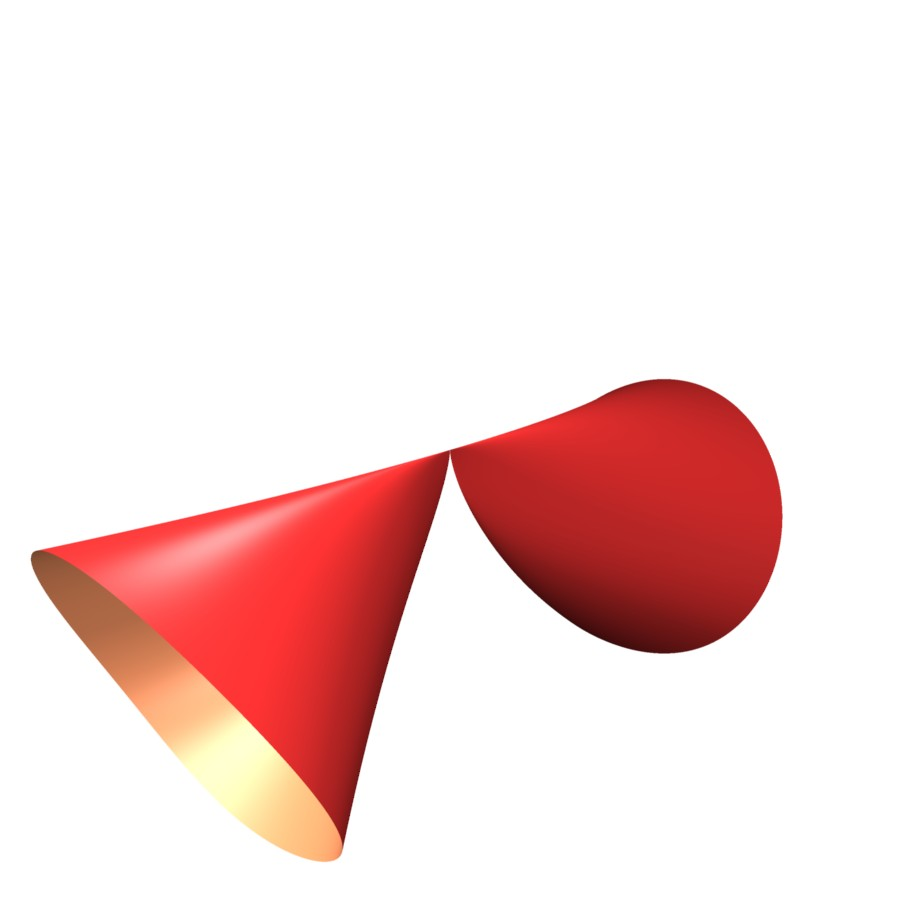
\includegraphics[width=1.1cm]{../../common/images/D5mm_01}\quad%
		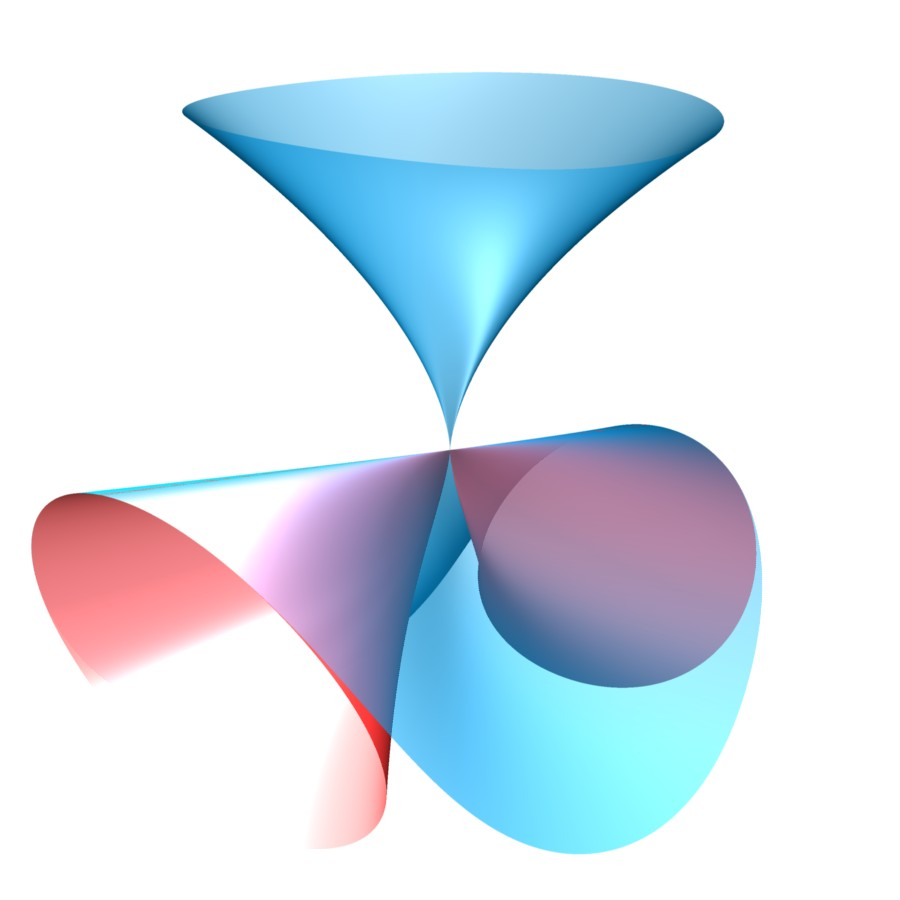
\includegraphics[width=1.1cm]{../../common/images/D5pm_D5mm}\quad%
		
\includegraphics[width=1.1cm]{../../common/images/D5pm_blue}%
	\end{Centering*}
	There also exist deformations between the $D_5^{--}$ and $D_4^{--}$ singularity, just like between the $D_5^{+-}$ and $D_4^{+-}$. The $D_5^{--}$ develops from the $D_4^{--}$ by shrinking the upper part until it is reduced to a point:
	\begin{Centering*}%
		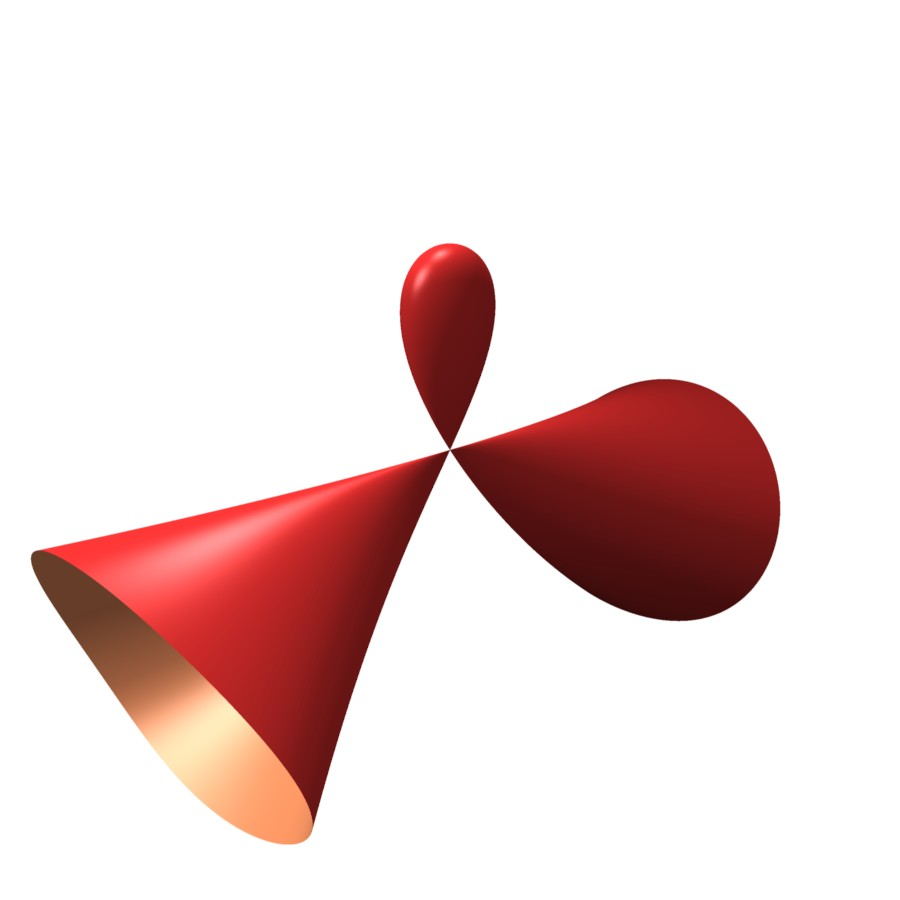
\includegraphics[width=1.1cm]{../../common/images/D5mm_03}\quad%
		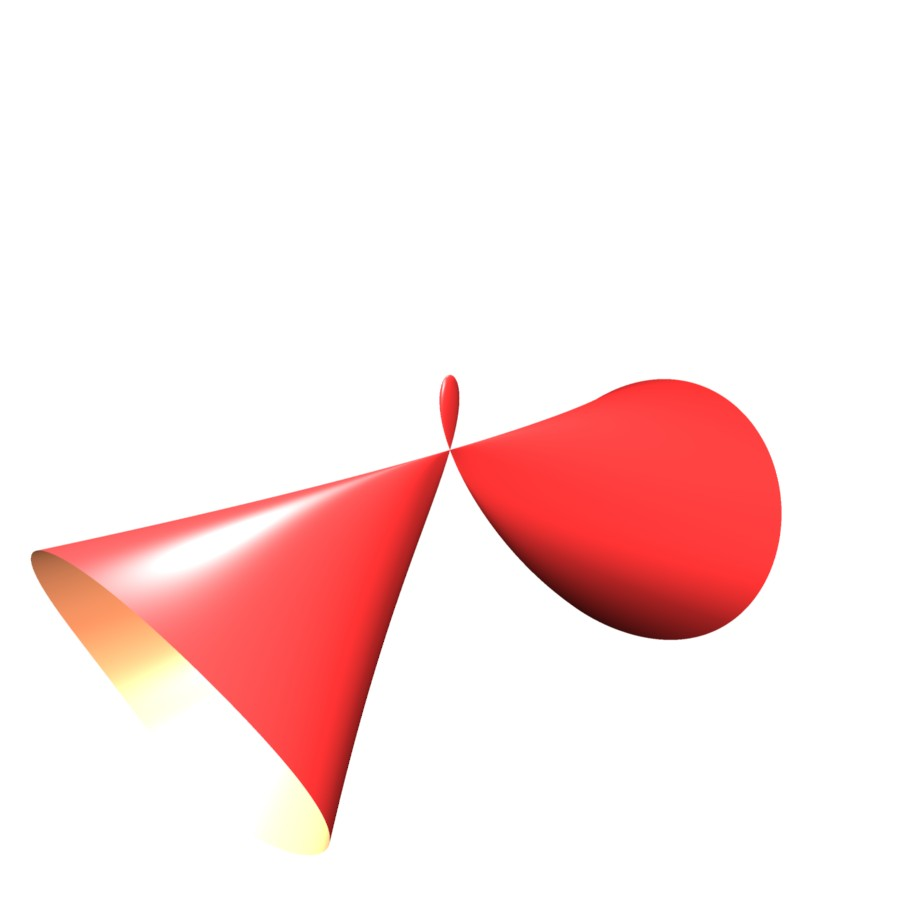
\includegraphics[width=1.1cm]{../../common/images/D5mm_02}\quad%
		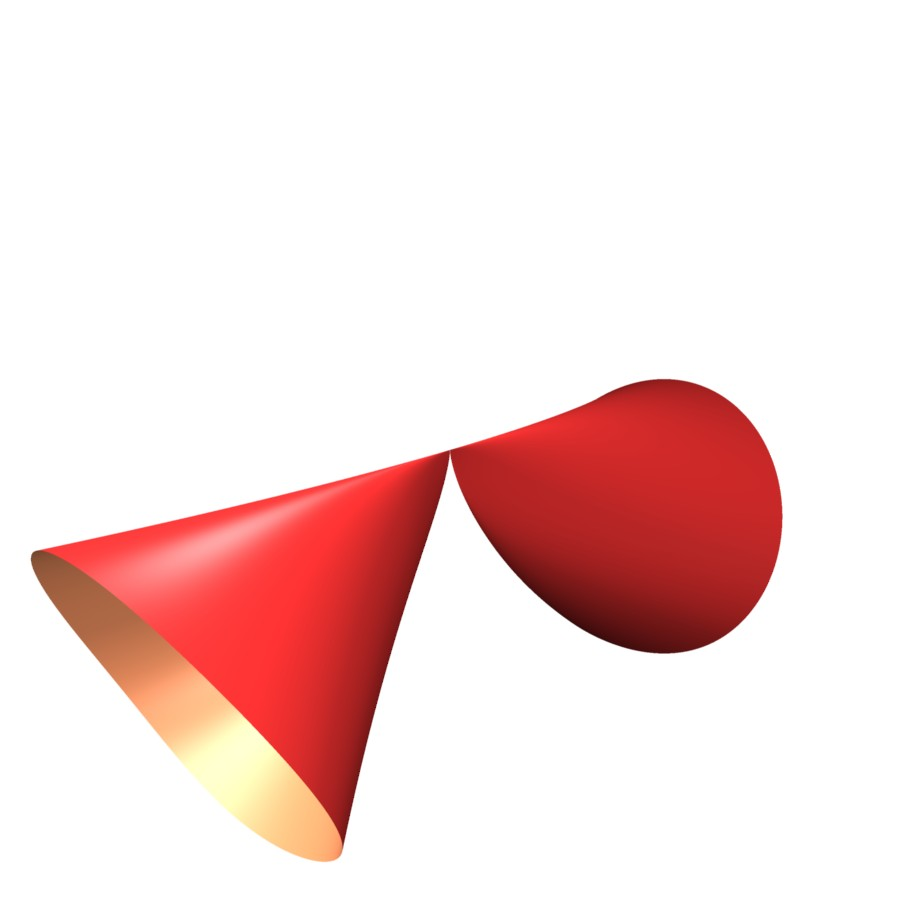
\includegraphics[width=1.1cm]{../../common/images/D5mm_01}%
	\end{Centering*}
	We can also make two $A_1$ and one $A_2$ singularities appear when deforming in another way:
	\begin{Centering*}%
		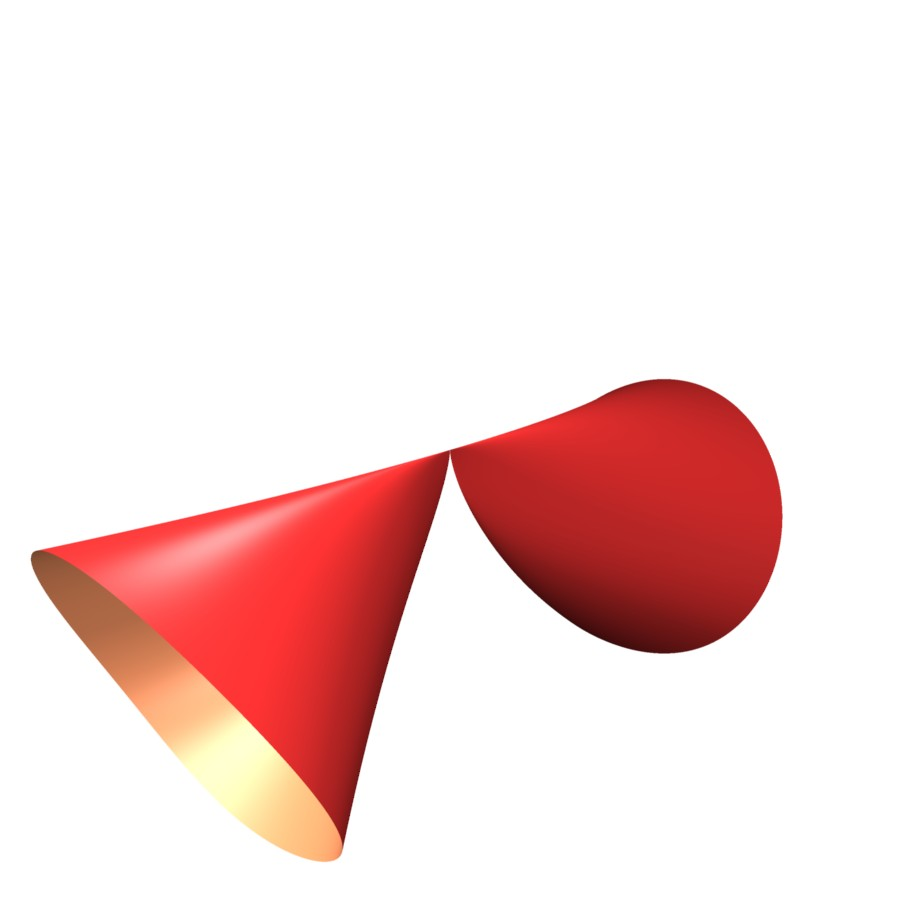
\includegraphics[width=1.1cm]{../../common/images/D5mm_01}\quad%
		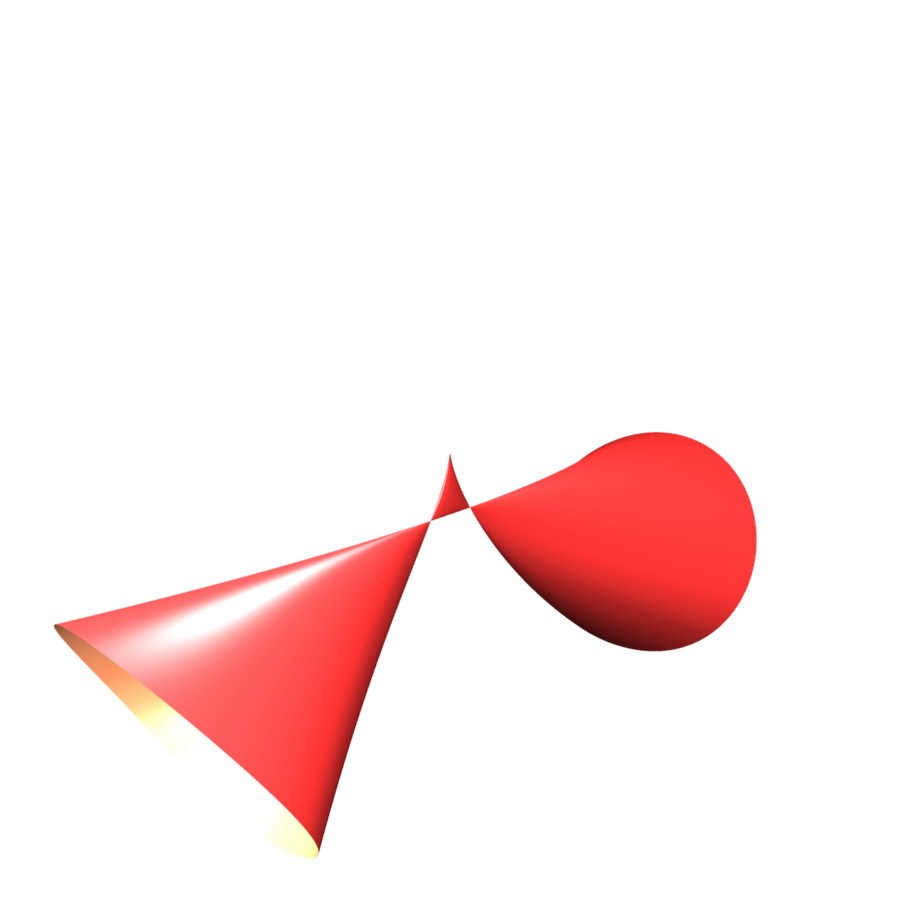
\includegraphics[width=1.1cm]{../../common/images/D5mm_04}\quad%
		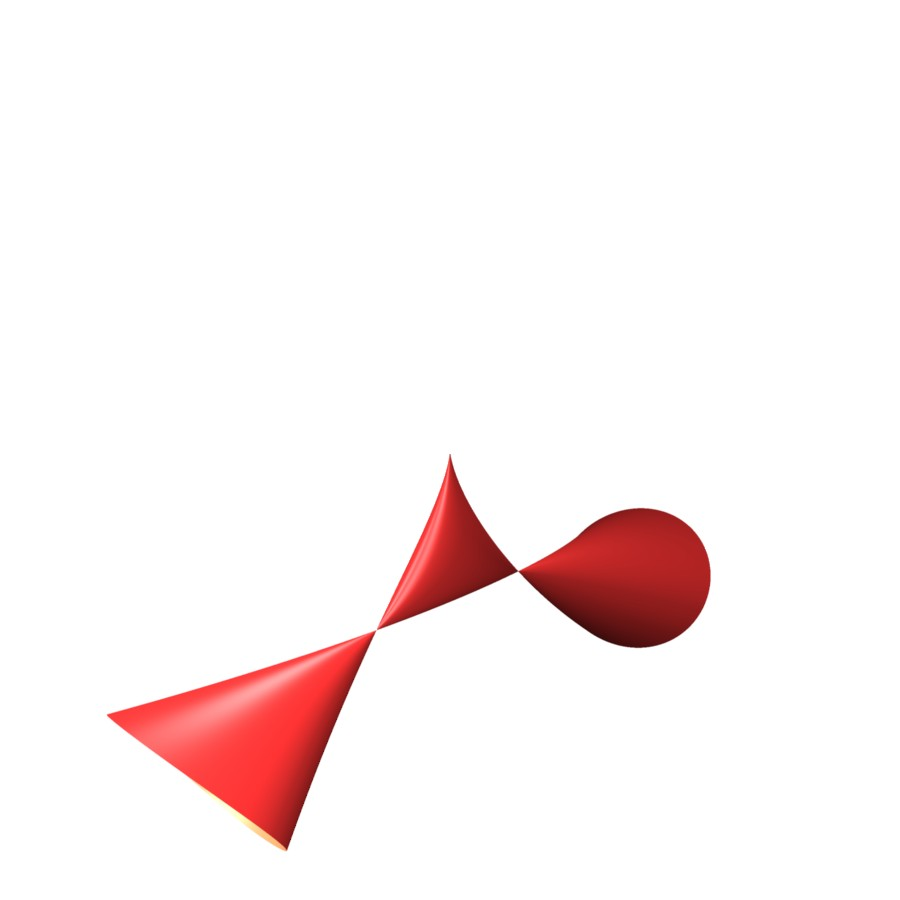
\includegraphics[width=1.1cm]{../../common/images/D5mm_05}%
	\end{Centering*}
\end{surferPage}
